\documentclass[crop,tikz]{standalone}

\usepackage{amsmath}
\tikzset{>=latex}
\newcommand{\F}{\vec{F}}

\begin{document}
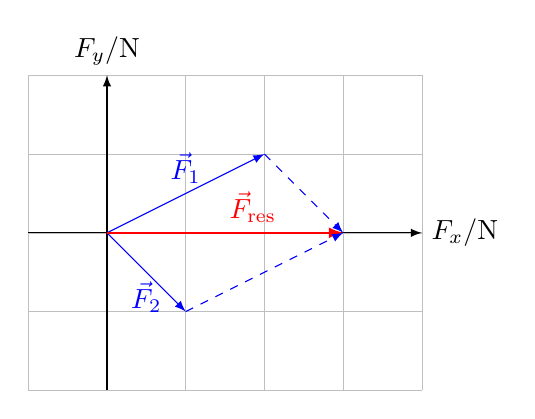
\begin{tikzpicture}
  \draw[step=1.0,gray!50,very thin] (-1,-2) grid (4,2);
  \draw[->] (-1,0) -- (4,0) node[right] {$F_x/\text{N}$};
  \draw[->] (0,-2) -- (0,2) node[above] {$F_y/\text{N}$};
  % 
  \draw[->,blue] (0,0) -- node[above] {$\F_1$} (2,1);
  \draw[->,blue] (0,0) -- node[below] {$\F_2$} (1,-1);
  \draw[->,red,thick] (0,0) -- node[above,xshift=1em] {$\F_\text{res}$} (3,0);
  \draw[->,blue,dashed] (2,1) -- (3,0);
  \draw[->,blue,dashed] (1,-1) -- (3,0);
\end{tikzpicture}
\end{document}
